
\medskip
\begin{minipage}[t]{0.5\linewidth}
	La figure ci-contre n'est pas en vraie grandeur.
	On donne les informations suivantes :
	\begin{itemize}
		\item Le triangle ADE a pour dimensions :
		
			AD = 7 cm, AE = 4,2 cm et DE = 5,6 cm.
		
		\item F est le point de [AD] tel que AF = 2,5 cm.
		\item B est le point de [AD) et C est le point de [AE) tels que : AB = AC = 9 cm.
		\item La droite (FG) est parallèle à la droite (DE).
	\end{itemize}

\smallskip

	\begin{enumerate}
		\item Réaliser une figure en vraie grandeur.
		\item Prouver que ADE est un triangle rectangle en E.
		\item Calculer la longueur FG.
	\end{enumerate}
\end{minipage}
\hfill
\begin{minipage}[t]{0.45\linewidth}
	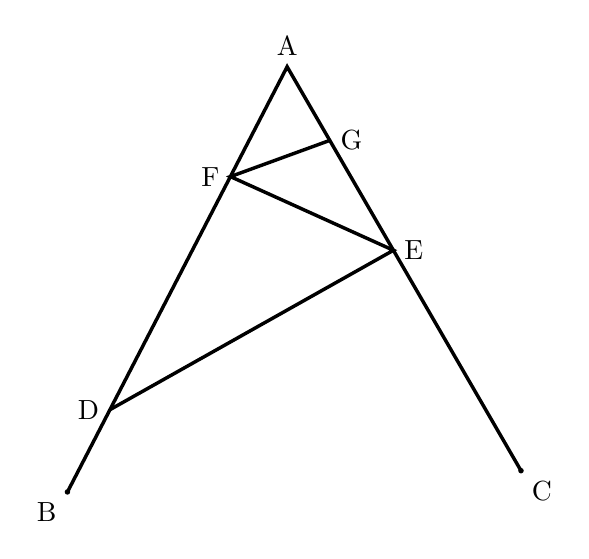
\begin{tikzpicture}[baseline = {(current bounding box.north)},x = 0.9cm,y=0.9cm,line width = 1.25pt]
	\draw (0,0) -- (3.1,6) -- (6.4,0.3);
	\draw (0.6,1.161) -- (4.6,3.41) -- (2.3,4.45) -- (3.7,4.96);
	\node at (0,0) [below left ]{B};
	\node at (0.6,1.161) [left] {D};
	\node at (2.3,4.45) [left] {F};
	\node at (3.1,6) [above] {A};
	\node at (3.7,4.96) [right] {G};
	\node at (4.6,3.41) [right] {E};
	\node at (6.4,0.3) [below right] {C};
	\fill (6.4,0.3) circle (1pt);
	\fill (0,0) circle (1pt);
	\end{tikzpicture}
\end{minipage}


